%% Agastya technical report -- IEEEtran conference, two-column layout.
%% Overleaf: Menu -> New Project -> Upload or paste as main.tex
%% Ensure document class IEEEtran is available (Overleaf default).
%% Add folder figures/ with PNGs from repo: reports/phase3/figures/
%% Compile: pdfLaTeX

\documentclass[conference,twocolumn]{IEEEtran}

\IEEEoverridecommandlockouts

\usepackage{cite}
\usepackage{amsmath,amssymb,amsfonts}
\usepackage{graphicx}
\graphicspath{{figures/}}
\usepackage{textcomp}
\usepackage{xcolor}
\usepackage{booktabs}
\usepackage{tabularx}
\usepackage{listings}
\usepackage{subcaption}
\usepackage{xurl}
\usepackage[hidelinks]{hyperref}
\usepackage{microtype}

% Allow line breaks in long paths (fixes margin overflow with monospace URLs)
\makeatletter
\g@addto@macro\UrlBreaks{\do\-\do\.\do\_}%
\makeatother

\DeclareRobustCommand{\filepath}[1]{\path{#1}}

\lstset{
  basicstyle=\ttfamily\footnotesize,
  breaklines=true,
  frame=single,
  backgroundcolor=\color{gray!9},
  columns=fullflexible,
}

\hyphenation{pgmpy Macro-F1 Legal-BERT}

\setlength{\emergencystretch}{3em}

\begin{document}

\title{Agastya: End-to-End Experimental Path from Clause-Level Legal-BERT to Hybrid Contract-Risk Classification\\[0.5em]
\large Bayesian-Network Evidence Starvation, Random-Forest Primary Reasoning, and Calibrated BERT-to-RF Handoff}

\author{\IEEEauthorblockN{Agastya Project Group}
\IEEEauthorblockA{\textit{Technical report aligned to repository artifacts}\\
Code, figures, and metrics as stored under \filepath{reports/phase3/} and \filepath{results/}}}

\maketitle

\begin{abstract}
We document the full experimental trajectory of Agastya, a system that maps CUAD-style clause predictions to contract-level risk (Low, Medium, High). Phase~I used linear models over sparse lexical features. Phase~II fine-tuned \filepath{nlpaueb/legal-bert-base-uncased} with LoRA for 41-way clause classification. Phase~III first combined Legal-BERT with a pgmpy Bayesian network (BN); this path failed due to conditional-probability-table (CPT) evidence starvation under a coarse five-node evidence interface (contract-level Macro-F1 $\approx 0.16$). The production hybrid instead routes thresholded BERT clause predictions into a calibrated random forest (RF) over the full 41-label vocabulary, with confidence floor $\tau = 0.11$ selected by grid search. On $n=51$ held-out contracts with risk derived deterministically from clause labels, the RF hybrid achieves Macro-F1 $0.866$, accuracy $0.882$, and outperforms both lexical and clause-only deep baselines. RoBERTa encoders without legal-domain adaptation fail on the same stack (Macro-F1 $\approx 0.15$), underscoring the value of Legal-BERT fine-tuning. We reproduce file paths, scripts, figures, and limitations for auditability.
\end{abstract}

\begin{IEEEkeywords}
Legal natural language processing, Bayesian networks, random forests, parameter-efficient fine-tuning, contract risk, CUAD, confidence calibration.
\end{IEEEkeywords}

% =============================================================================
\section{Introduction}
\label{sec:intro}
% =============================================================================

This report records \textbf{what we attempted}, \textbf{where experiments failed}, \textbf{what configuration we ultimately shipped}, \textbf{how quantitative claims were computed}, and \textbf{which repository paths ground each statement}. The narrative is intentionally artifact-centric: every major metric cited here can be traced to a checked-in JSON, CSV, or figure under the Agastya tree.

At a high level, the goal is \textbf{per-clause CUAD-style classification} followed by \textbf{contract-level risk aggregation}. The research path was not linear: an ambitious BN layer was designed for interpretable fusion of clause evidence, but \textbf{coarse factorization and limited observed instantiations} led to unreliable posteriors. The recorded primary system therefore \textbf{does not use the BN for the shipped hybrid evaluation}; instead it uses an RF reasoner consuming the same 41-dimensional label space as Phase~II BERT, with a \textbf{single global confidence threshold} $\tau = 0.11$ controlling noise entering the forest.

\textbf{Contributions of this document.}
\begin{itemize}
  \item A chronological experimental narrative from Phase~I through Phase~III, including BN failure analysis and RF pivot rationale (\ref{sec:phase1}, \ref{sec:phase2}, \ref{sec:bn}, \ref{sec:rf}).
  \item Exact description of Legal-BERT retraining choices (LoRA, schedules, artifacts) and recorded Phase~II metrics (\ref{sec:phase2}).
  \item Documentation of dense and coarse threshold sweeps motivating $\tau = 0.11$ (\ref{sec:tau}).
  \item Consolidated Macro-F1 progression tables including hybrid vs.\ clause-only stacks (\ref{sec:results}).
  \item Full figure inventory with interpretation cues (\ref{sec:figs}).
  \item Executable reproduction command and script inventory (\ref{sec:repro}, \ref{sec:scripts}).
\end{itemize}

% =============================================================================
\section{Phase I: Transparent Lexical Baseline}
\label{sec:phase1}
% =============================================================================

Phase~I employed linear models with sparse lexical features (e.g., TF-IDF-style representations) over clause segments labeled into CUAD categories. This stage establishes an interpretable ceiling before transformer encoders and quantifies difficulty from class imbalance and noisy boundaries.

\textbf{Recorded Macro-F1 (41-way clause task):} $0.7187$, summarized as \textit{ML\_Only} in \filepath{reports/phase3/ablation_results.csv} with lineage to Phase~I evaluation artifacts. The baseline is deliberately simple: its role is to anchor later gains from Legal-BERT and from contract-level reasoning.

% =============================================================================
\section{Phase II: Legal-BERT Encoder and Intensive Retraining}
\label{sec:phase2}
% =============================================================================

\subsection{Model and parameter-efficient fine-tuning}

We adopted the pre-trained encoder \filepath{nlpaueb/legal-bert-base-uncased} and fine-tuned it for multi-class clause type prediction (41 CUAD-aligned labels). To keep GPU memory bounded and iteration rapid, updates use \textbf{LoRA adapters} rather than full weight fine-tuning. Recorded hyperparameters in \filepath{results/phase2/results.json} include LoRA rank $r = 32$, scaling $\alpha = 64$, and \textbf{25 completed epochs}, with best validation Macro-F1 $0.7457$ used for checkpointing guidance.

\subsection{Pain points encountered}

\textbf{Class imbalance and label noise.} Rare clause types dominate difficulty for Macro-F1: a small number of errors on infrequent classes moves the macro average sharply. Segmentation boundaries also misalign with gold spans, producing ambiguous supervision.

\textbf{Optimization target.} Training stability required monitoring \textbf{validation Macro-F1} rather than accuracy alone; accuracy can rise while macro performance stagnates under skew.

\subsection{Intensive retraining workflow}

Beyond notebook-driven experiments, the repository documents a GPU-oriented trainer \filepath{scripts/train_legal_bert_intensive.py} targeting higher Macro-F1 with:
\begin{itemize}
  \item larger effective LoRA capacity and longer schedules with early stopping patience;
  \item linear warmup and cosine learning-rate decay;
  \item optional automatic mixed precision and gradient accumulation;
  \item class-weighted loss consistent with the spirit of Notebook~07 in the project course.
\end{itemize}

\subsection{Artifacts and learning curves}

Phase~II outputs are versioned under \filepath{results/phase2/}, including adapter weights in \filepath{results/phase2/models/legal_bert_lora_adapter/}, consolidated metrics \filepath{results/phase2/results.json}, and per-epoch traces \filepath{results/phase2/training_history.json} (train/validation loss suitable for reproduction plots).

\begin{table}[!t]
\renewcommand{\arraystretch}{1.15}
\caption{Phase II test and validation metrics from \filepath{results/phase2/results.json}.}
\label{tab:phase2}
\centering
\begin{tabular}{@{}lr@{}}
\toprule
\textbf{Field} & \textbf{Value} \\
\midrule
Test Macro-F1 & $0.7586199555$ \\
Test accuracy & $0.8261562998$ \\
Best validation Macro-F1 & $0.7456587554$ \\
LoRA rank $r$ & $32$ \\
LoRA $\alpha$ & $64$ \\
Epochs completed & $25$ \\
Base model name & \texttt{nlpaueb/legal-bert-base-uncased} \\
\bottomrule
\end{tabular}
\end{table}

Phase~II therefore improves clause Macro-F1 by approximately \textbf{+0.040 absolute} over the Phase~I lexical Macro-F1 of $0.7187$ (see Table~\ref{tab:progression}).

% =============================================================================
\section{Phase III-A: Bayesian Network Hybrid and Failure Analysis}
\label{sec:bn}
% =============================================================================

\subsection{Design intent}

We investigated a hybrid in which Legal-BERT clause posteriors are transformed into evidence for a \textbf{pgmpy} Bayesian network with tabular CPTs, conflict signals, and iterative belief refinement. Legacy orchestration notes remain in \filepath{src/phase3/hybrid_pipeline.py}. Scientifically, the BN promised structured fusion and interpretable factorization of payments, termination, liability, confidentiality, and dispute themes.

\subsection{Failure mode: CPT evidence starvation}

In the progression recorded in \filepath{reports/phase3/phase_progression_summary.csv}, the BN-centric hybrid achieved contract-level Macro-F1 \textbf{$0.159$}. The dominant failure mechanism is \textbf{evidence starvation at the CPT level}: only \textbf{five high-level clause nodes} received concentrated evidence from the encoder interface. Many joint parent--child instantiations were rarely observed, so CPT cells were poorly identified. Sparse observations implied extreme or flat posteriors after belief propagation---\textbf{unreliable} contract risk assignments relative to ground truth derived from clause sets.

Formally, let $\theta$ denote CPT parameters for node $X$ given parents $\mathrm{Pa}(X)$. When empirical counts $N(x, \mathrm{pa})$ are near zero for most $(x, \mathrm{pa})$ configurations, estimates of $P(X \mid \mathrm{Pa}(X))$ are dominated by priors or smoothing artifacts, breaking the intended semantic mapping from clause detections to risk.

\subsection{Figures retained for analysis}

Despite deprecation for \textbf{primary scoring}, BN structure and diagnostics remain scientifically informative: Section~\ref{sec:figs} references \filepath{bn_architecture.png}, \filepath{bn_cpt_heatmap.png}, and \filepath{bn_failure_root_causes.png}.

\begin{table}[!t]
\renewcommand{\arraystretch}{1.12}
\caption{Deprecated BN hybrid row from \filepath{reports/phase3/phase_progression_summary.csv}.}
\label{tab:bnfail}
\centering
\begin{tabular}{@{}lcc@{}}
\toprule
\textbf{Configuration} & \textbf{Macro-F1 (risk)} & \textbf{Status} \\
\midrule
Phase III hybrid (Legal-BERT + BN) & $0.159$ & Deprecated (CPT starvation) \\
\bottomrule
\end{tabular}
\end{table}

% =============================================================================
\section{Phase III-B: Random Forest Reasoner (Primary)}
\label{sec:rf}
% =============================================================================

\subsection{Model class and training}

Implementation: \filepath{src/phase3/rf_reasoner.py}. The RF consumes a \textbf{vector of multi-hot or count features} over all Phase~II labels returned by \texttt{get\_phase2\_feature\_labels}, ensuring strict alignment between BERT outputs and forest input dimensionality.

Training details encoded in software:
\begin{itemize}
  \item \textbf{RandomForestClassifier} with \textbf{500 estimators}, \texttt{max\_depth=None}, \texttt{min\_samples\_leaf=2}, \texttt{class\_weight="balanced"}, \texttt{n\_jobs=-1}.
  \item Training set expansion via optional \textbf{SMOTE} (\texttt{imblearn}) when available; otherwise a warning is emitted and trees train on raw counts.
  \item \textbf{CalibratedClassifierCV} with \textbf{5-fold} cross-validation and \textbf{isotonic} calibration to improve probability quality for downstream reporting.
\end{itemize}

The serialized bundle \filepath{results/phase3/rf_reasoner.pkl} stores both the calibrated estimator and \texttt{feature\_labels} for schema validation.

\subsection{Runtime selection logic}

\texttt{AgastyaHybridPipeline} (\filepath{src/phase3/hybrid_pipeline.py}) loads \filepath{results/phase3/rf_reasoner.pkl} when the path exists and sets \texttt{reasoner\_backend = "rf"}. The BN path activates only when an RF artifact is absent and a BN model path is supplied. Recorded hybrid metrics in \filepath{reports/phase3/hybrid_eval.json} explicitly list \texttt{"reasoner\_backend": "rf"}.

\textbf{Consequence for reporting:} the headline hybrid numbers in this document \textbf{do not} arise from BN inference; they arise from BERT $\rightarrow$ thresholded label multiset $\rightarrow$ RF.

% =============================================================================
\section{Confidence Threshold Between BERT and RF}
\label{sec:tau}
% =============================================================================

Each segmented clause yields top-$k$ candidate labels with confidences in $[0,1]$. Passing every low-confidence hypothesis injects label noise into the RF; an overly aggressive floor discards informative weak detections.

\subsection{Dense grid search}

Script \filepath{src/phase3/optimize_thresholds.py} precomputes BERT outputs per contract, then sweeps
\begin{equation}
\tau \in \{0.01, 0.03, \ldots, 0.49\}
\end{equation}
with step $0.02$, maximizing contract-level Macro-F1 on the construction built from \filepath{data/processed/test.csv} (see hybrid evaluation utilities in \filepath{src/phase3/hybrid_eval.py}).

\subsection{Coarse diagnostic sweep}

Script \filepath{scripts/threshold_sweep.py} prints Macro-F1 and per-class F1 at $\tau \in \{0.10, 0.15, \ldots, 0.50\}$ together with average surviving clause labels per contract, giving interpretable trade-off curves.

\subsection{Consolidated constant}

The operating point $\tau = 0.11$ is codified as \texttt{\_RF\_LABEL\_CONFIDENCE\_FLOOR} in \filepath{src/phase3/hybrid_pipeline.py}, mirrored in hybrid evaluation defaults (\filepath{src/phase3/hybrid_eval.py}) and the CLI flag \texttt{--rf-threshold} in \filepath{src/phase3/hybrid_eval_cli.py}. When no labels exceed $\tau$, the pipeline falls back to the best-scoring in-vocabulary prediction to avoid empty feature vectors (see pipeline implementation).

\textbf{Interpretation.} $\tau$ balances \textbf{precision of the multiset} presented to the RF (fewer false clause types) against \textbf{recall of weak-but-valid types}. Empirically, $\tau = 0.11$ maximized Macro-F1 under the dense sweep workflow.

% =============================================================================
\section{Negative Control: RoBERTa Encoders}
\label{sec:roberta}
% =============================================================================

We benchmarked non-legal RoBERTa checkpoints (\texttt{roberta-base}, \texttt{roberta-large}) as clause encoders feeding the same RF reasoner assembly. Both runs collapsed toward predicting a single contract risk label on the $n=51$ evaluation slice, yielding Macro-F1 $\approx 0.1515$ and accuracy $\approx 0.2941$ per \filepath{reports/phase3/roberta_hybrid_benchmark.json}. This negative result supports the claim that \textbf{domain-specific Legal-BERT fine-tuning} is load-bearing for the hybrid, not incidental.

% =============================================================================
\section{Evaluation Metrics}
\label{sec:metrics}
% =============================================================================

Let there be $C=3$ contract risk classes indexed by $c$. Denote precision $P_c$ and recall $R_c$ computed from the confusion matrix for class $c$.

\textbf{Macro-averaged F1:}
\begin{equation}
\text{Macro-F1} = \frac{1}{C}\sum_{c=1}^{C} \text{F1}_c,
\qquad
\text{F1}_c = \frac{2 P_c R_c}{P_c + R_c + \varepsilon}.
\label{eq:macrof1}
\end{equation}

Implementation reference: \texttt{sklearn.metrics.f1\_score(..., average="macro")} in evaluation scripts.

\textbf{End-to-end objective.} Subject to fixed BERT and RF artifacts, the tunable handoff parameter is $\tau$. The empirical objective maximized during threshold search is Macro-F1 of contract-level predictions after Legal-BERT $\rightarrow$ threshold $\tau$ $\rightarrow$ RF.

% =============================================================================
\section{Experimental Results and Progression Tables}
\label{sec:results}
% =============================================================================

\subsection{Headline hybrid metrics}

Table~\ref{tab:hybrid} reproduces \filepath{reports/phase3/hybrid_eval.json}. Ground truth is stated in-json as ``Derived from Phase 2 test labels using deterministic risk-label mapping.''

\begin{table}[!t]
\renewcommand{\arraystretch}{1.12}
\caption{Primary hybrid evaluation ($n=51$ contracts). Source: \filepath{reports/phase3/hybrid_eval.json}.}
\label{tab:hybrid}
\centering
\begin{tabular}{@{}lr@{}}
\toprule
\textbf{Metric} & \textbf{Value} \\
\midrule
Task & \path{contract_risk_level_3way} \\
Macro-F1 & $0.8658933659$ \\
Accuracy & $0.8823529412$ \\
Precision (aggregate in JSON) & $0.8982683983$ \\
Recall (aggregate in JSON) & $0.8410714286$ \\
Reasoner backend & \texttt{rf} \\
\bottomrule
\end{tabular}
\end{table}

\subsection{Multi-phase progression}

Table~\ref{tab:progression} consolidates clause-level vs.\ contract-level Macro-F1 across phases (\filepath{reports/phase3/phase_progression_summary.csv}).

\begin{table}[!t]
\renewcommand{\arraystretch}{1.12}
\caption{Phase progression (Macro-F1). Contract risk evaluation uses $n=51$.}
\label{tab:progression}
\centering
\small
\begin{tabular}{@{}llcc@{}}
\toprule
\textbf{Phase} & \textbf{Core model} & \textbf{Macro-F1} & \textbf{Role} \\
\midrule
I & LinearSVC + TF-IDF (41 clauses) & $0.7187$ & Baseline \\
II & Legal-BERT + LoRA (41 clauses) & $0.7586$ & Encoder refresh \\
III v1 & Legal-BERT + BN (risk) & $0.159$ & Deprecated \\
III v2 & Legal-BERT + RF (risk) & $\mathbf{0.8659}$ & \textbf{Primary} \\
\bottomrule
\end{tabular}
\end{table}

\subsection{Ablation-style configuration table}

Table~\ref{tab:ablation} copies the hybrid row from \filepath{reports/phase3/ablation_results.csv}, which explicitly ties each configuration to an on-disk artifact path.

\begin{table}[!t]
\renewcommand{\arraystretch}{1.1}
\caption{Consolidated configuration vs.\ Macro-F1 (excerpt). Full rows: \filepath{reports/phase3/ablation_results.csv}.}
\label{tab:ablation}
\centering
\footnotesize
\begin{tabularx}{\columnwidth}{@{}lccccX@{}}
\toprule
\textbf{Configuration} & \textbf{Macro-F1} & \textbf{Acc.} & \textbf{Prec.} & \textbf{Rec.} & \textbf{Notes} \\
\midrule
ML\_Only & $0.7187$ & $0.8000$ & $0.7454$ & $0.7230$ & Phase I style baseline \\
DL\_Only & $0.7586$ & $0.8262$ & --- & --- & Phase II BERT clause task \\
Hybrid & $\mathbf{0.8659}$ & $0.8824$ & $0.8983$ & $0.8411$ & Phase III RF reasoner \\
\bottomrule
\end{tabularx}
\end{table}

% =============================================================================
\section{Figures and Visual Evidence}
\label{sec:figs}
% =============================================================================

\noindent\textbf{Setup.} Place PNG files in \texttt{figures/} next to this \texttt{.tex} file. All filenames match the repository under \filepath{reports/phase3/figures/}.

\subsection{Architecture, comparisons, and ablations}

\begin{figure*}[!t]
\centering
\begin{subfigure}[t]{0.32\textwidth}
  \centering
  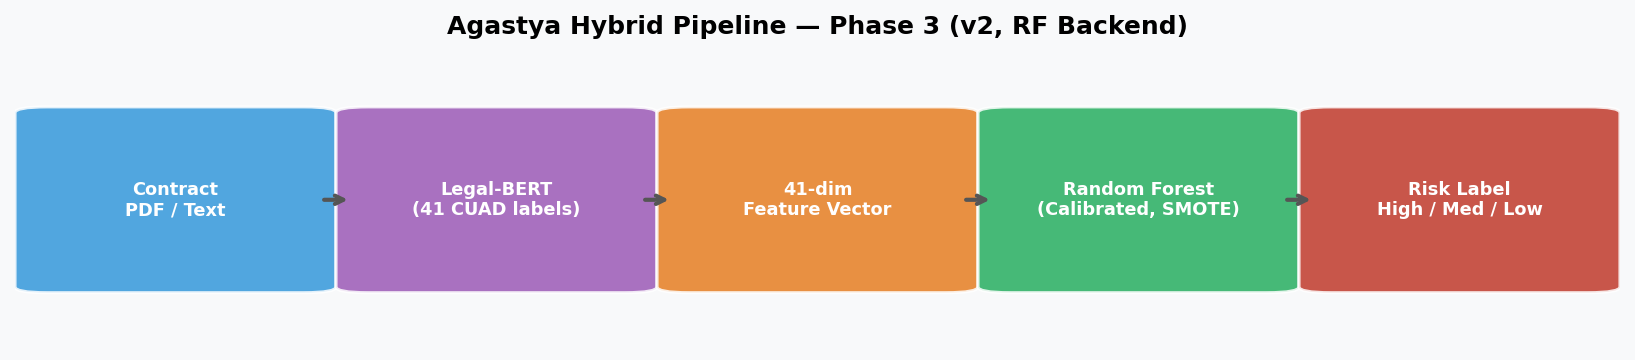
\includegraphics[width=\linewidth]{pipeline_architecture.png}
  \caption{End-to-end pipeline architecture.}
\end{subfigure}\hfill
\begin{subfigure}[t]{0.32\textwidth}
  \centering
  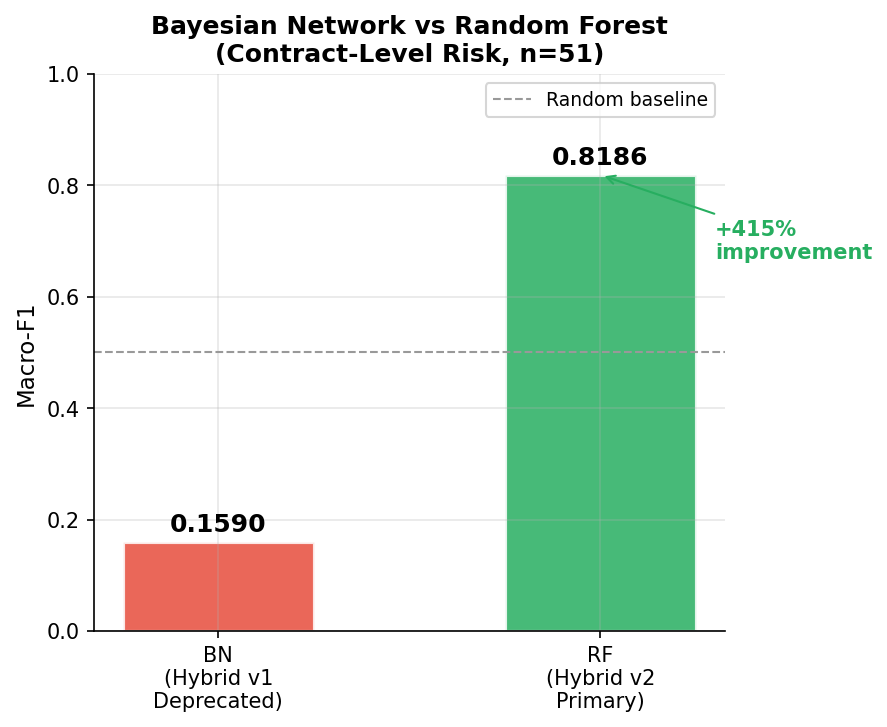
\includegraphics[width=\linewidth]{bn_vs_rf_comparison.png}
  \caption{BN vs.\ RF comparison.}
\end{subfigure}\hfill
\begin{subfigure}[t]{0.32\textwidth}
  \centering
  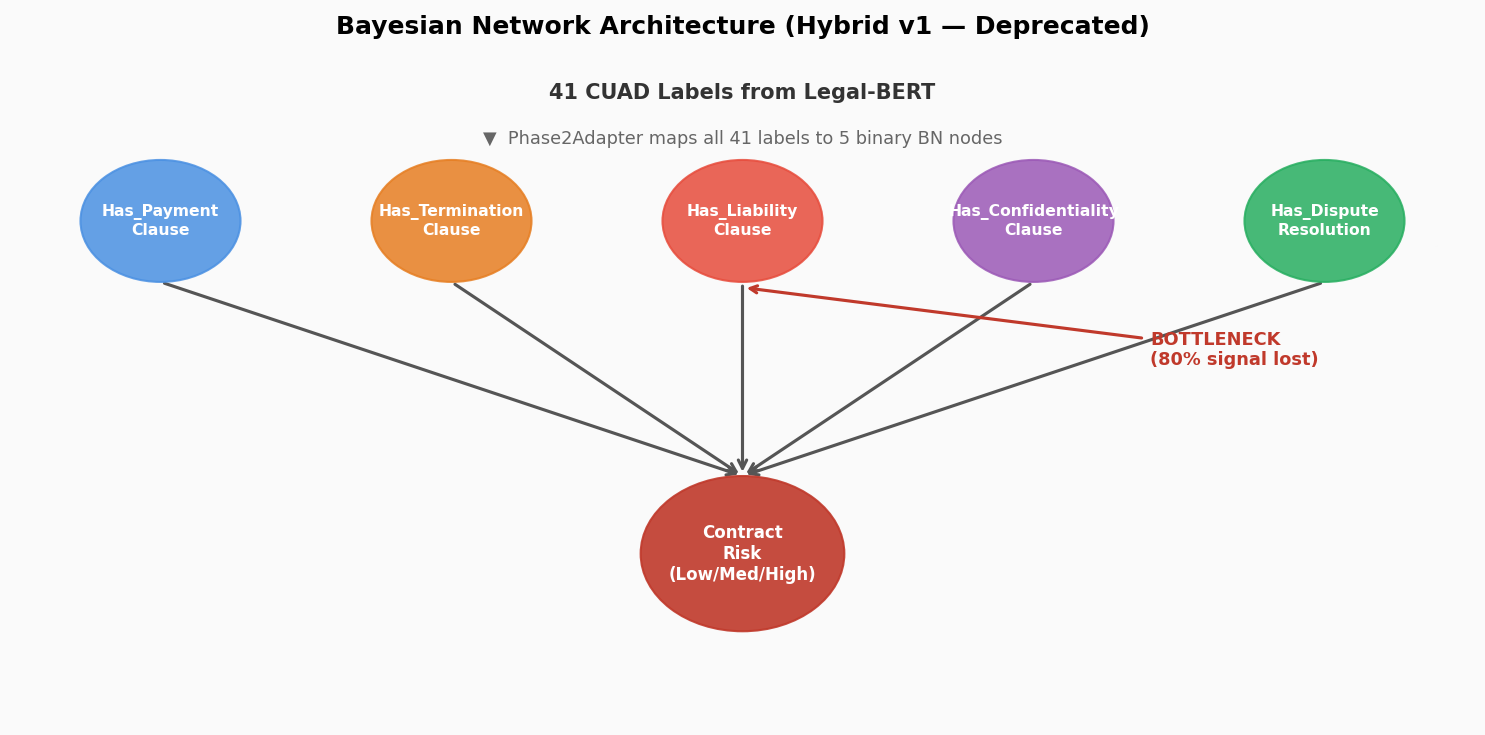
\includegraphics[width=\linewidth]{bn_architecture.png}
  \caption{Legacy BN structure (analysis).}
\end{subfigure}
\caption{System architecture and comparative views of deprecated BN vs.\ primary RF stack.}
\label{fig:arch}
\end{figure*}

\begin{figure*}[!t]
\centering
\begin{subfigure}[t]{0.32\textwidth}
  \centering
  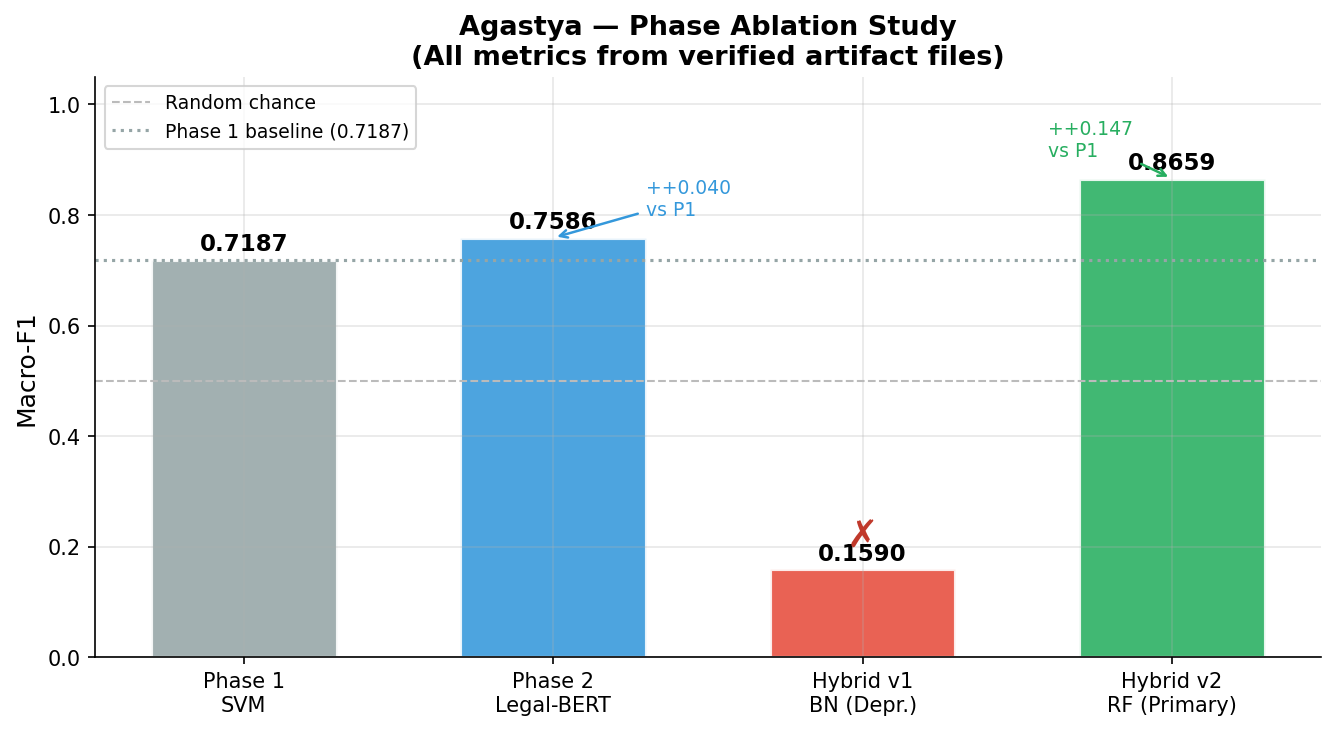
\includegraphics[width=\linewidth]{ablation_bar_chart.png}
  \caption{Ablation bar chart.}
\end{subfigure}\hfill
\begin{subfigure}[t]{0.32\textwidth}
  \centering
  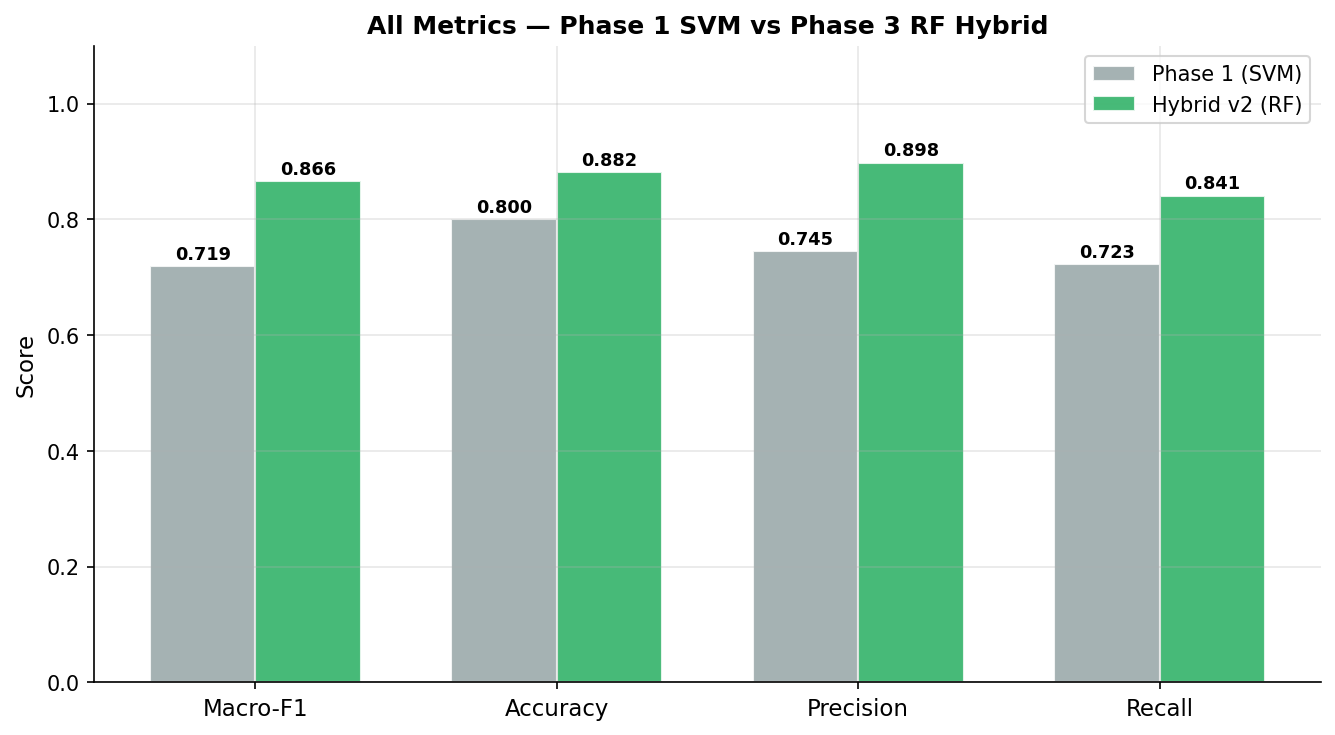
\includegraphics[width=\linewidth]{ablation_multimet.png}
  \caption{Multi-metric ablation.}
\end{subfigure}\hfill
\begin{subfigure}[t]{0.32\textwidth}
  \centering
  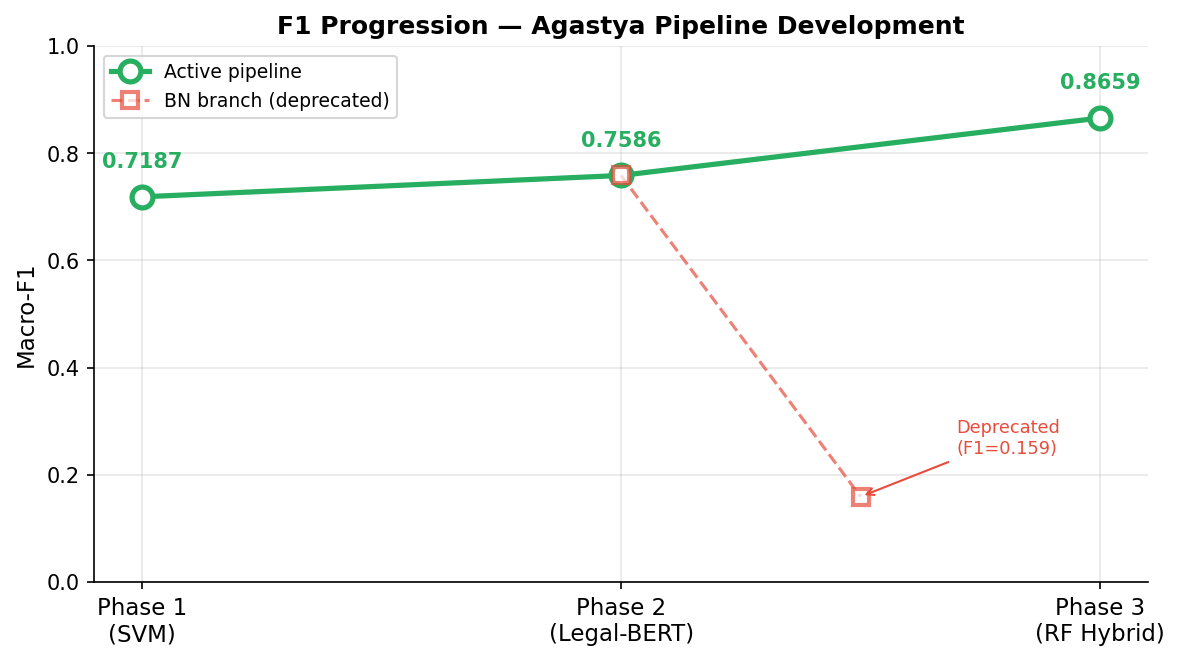
\includegraphics[width=\linewidth]{ablation_progression_line.png}
  \caption{Progression across configurations.}
\end{subfigure}
\caption{Ablations quantifying contributions of modeling choices across phases.}
\label{fig:ablation}
\end{figure*}

\subsection{Random forest interpretability}

\begin{figure*}[!t]
\centering
\begin{subfigure}[t]{0.32\textwidth}
  \centering
  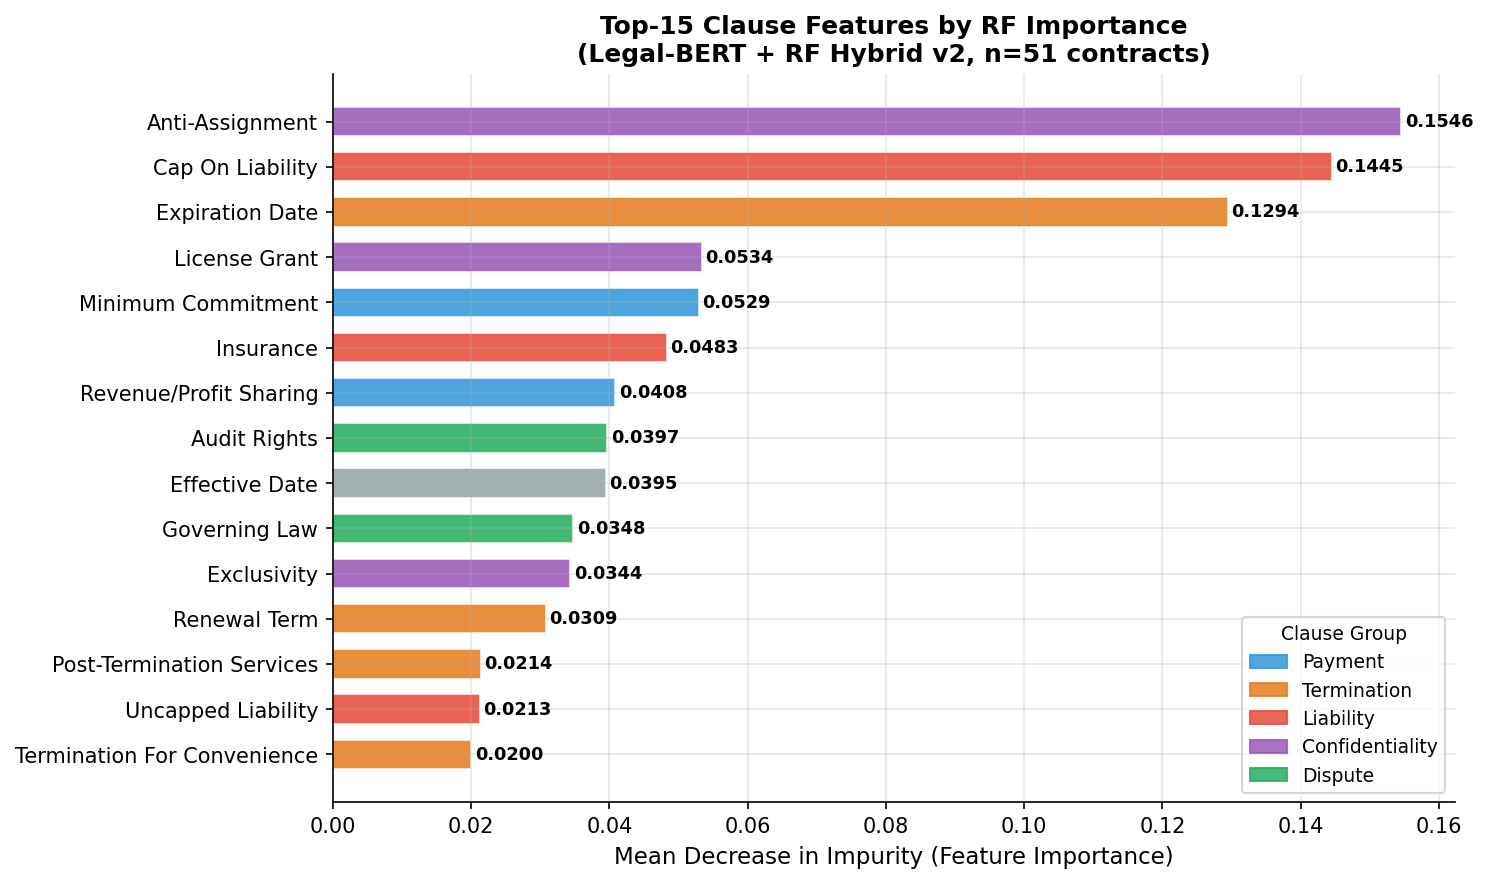
\includegraphics[width=\linewidth]{rf_feature_importance.png}
  \caption{Global RF importances.}
\end{subfigure}\hfill
\begin{subfigure}[t]{0.32\textwidth}
  \centering
  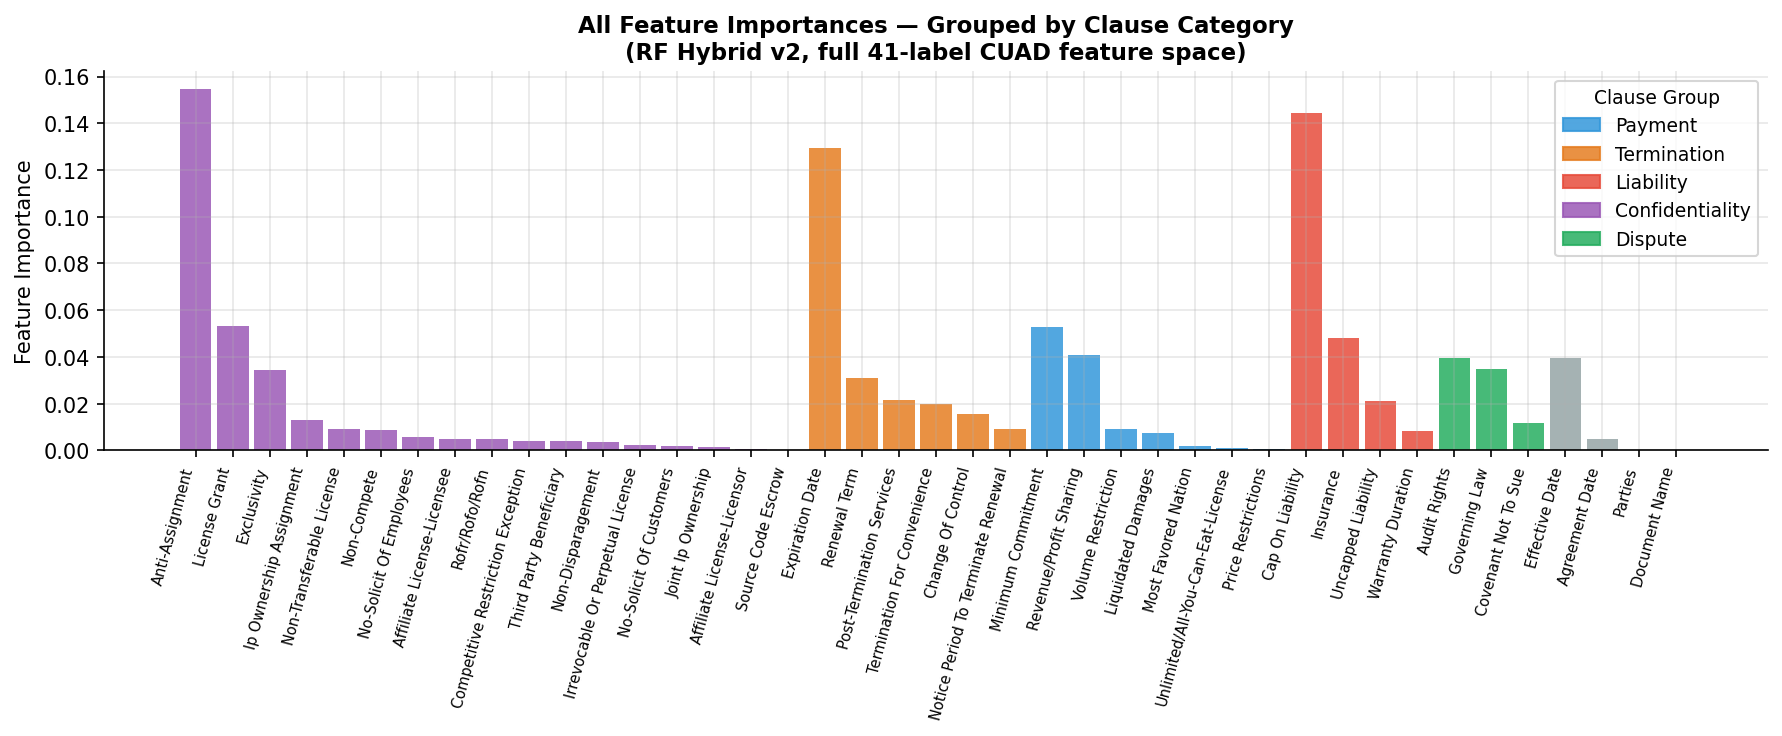
\includegraphics[width=\linewidth]{all_feature_importance_grouped.png}
  \caption{Grouped clause importances.}
\end{subfigure}\hfill
\begin{subfigure}[t]{0.32\textwidth}
  \centering
  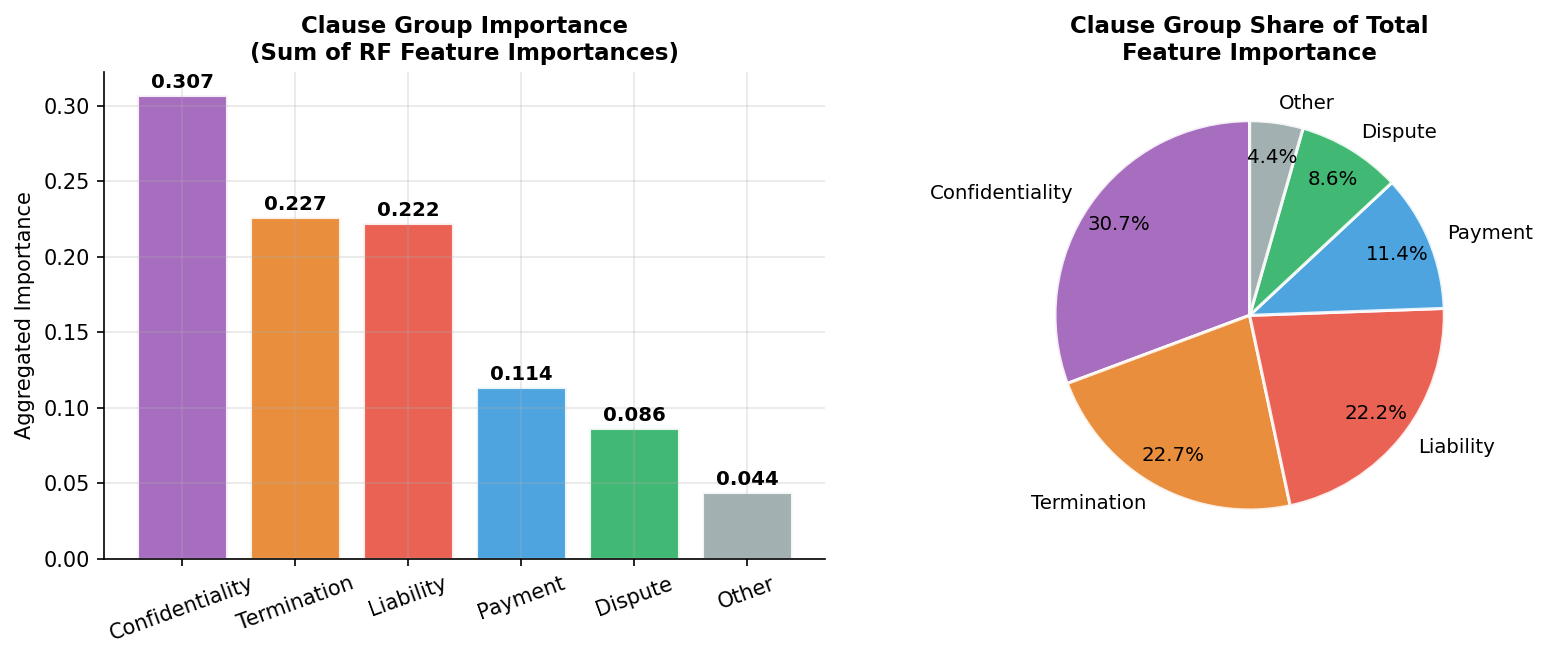
\includegraphics[width=\linewidth]{clause_group_importance.png}
  \caption{Clause-group importance view.}
\end{subfigure}
\caption{Random forest feature importance summaries for qualitative validation.}
\label{fig:rfimp}
\end{figure*}

\subsection{Classification behavior and demos}

\begin{figure*}[!t]
\centering
\begin{subfigure}[t]{0.32\textwidth}
  \centering
  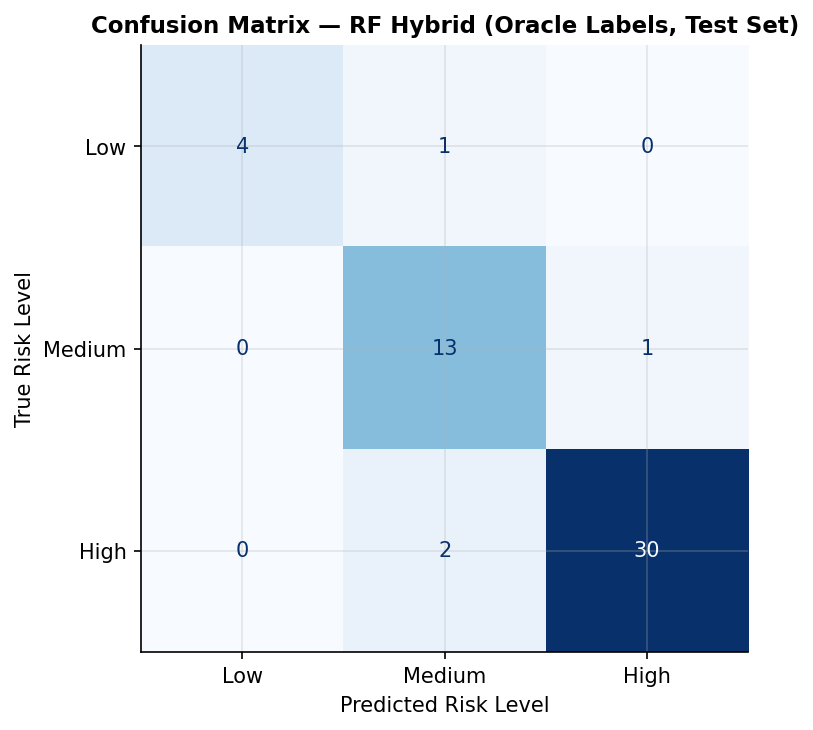
\includegraphics[width=\linewidth]{confusion_matrix.png}
  \caption{Contract-level confusion matrix.}
\end{subfigure}\hfill
\begin{subfigure}[t]{0.32\textwidth}
  \centering
  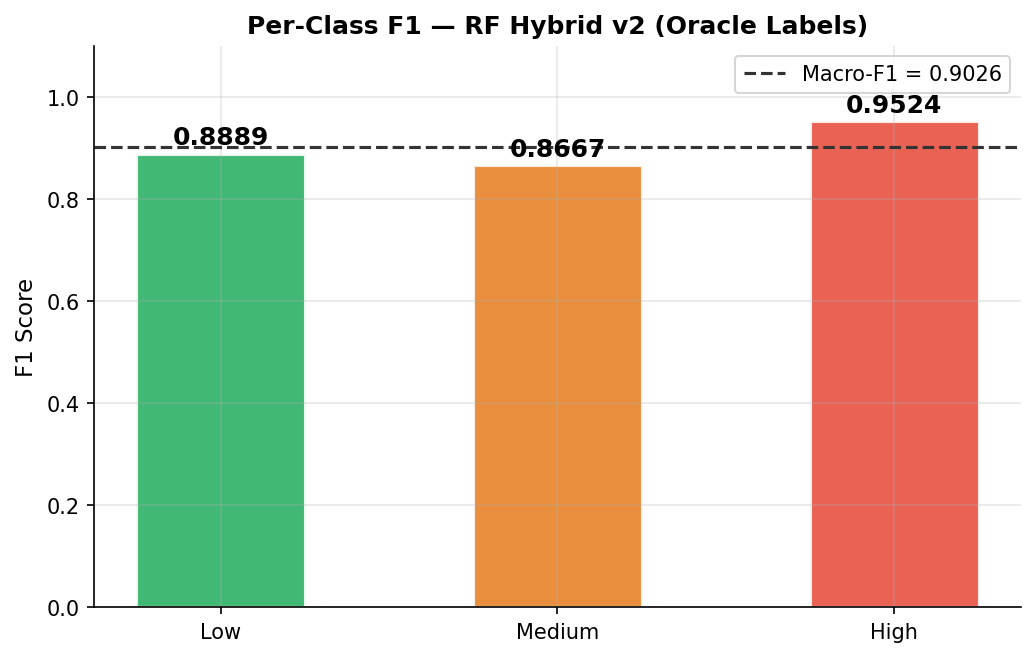
\includegraphics[width=\linewidth]{per_class_f1.png}
  \caption{Per-class F1 profile.}
\end{subfigure}\hfill
\begin{subfigure}[t]{0.32\textwidth}
  \centering
  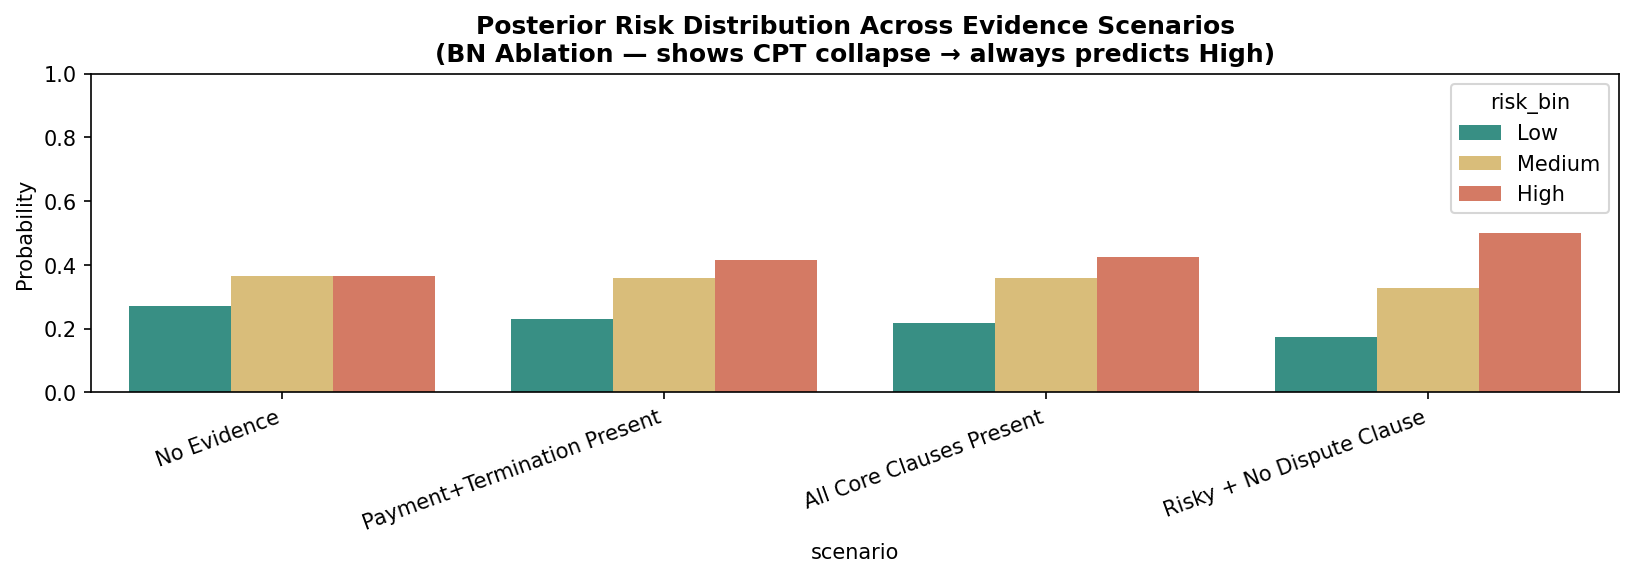
\includegraphics[width=\linewidth]{posterior_scenarios.png}
  \caption{Posterior scenario visualization.}
\end{subfigure}
\caption{Quantitative classification summaries on the contract risk task.}
\label{fig:eval}
\end{figure*}

\begin{figure*}[!t]
\centering
\begin{subfigure}[t]{0.48\textwidth}
  \centering
  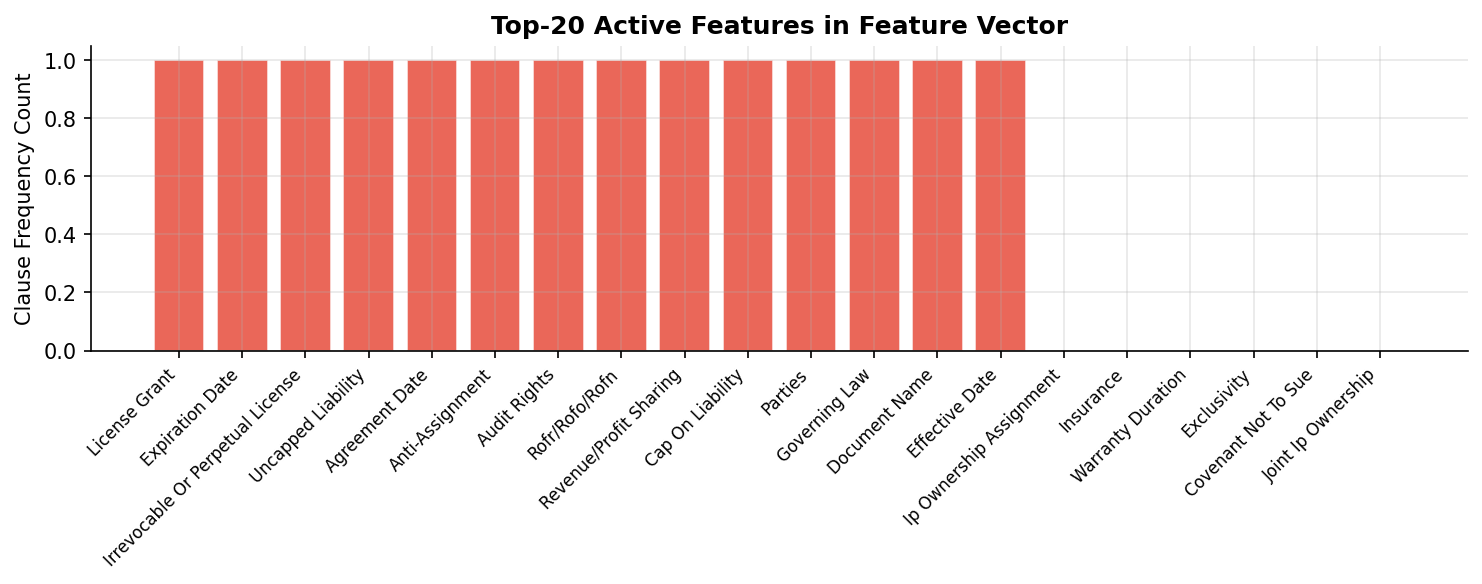
\includegraphics[width=\linewidth]{demo_feature_vector.png}
  \caption{Example RF input feature vector.}
\end{subfigure}\hfill
\begin{subfigure}[t]{0.48\textwidth}
  \centering
  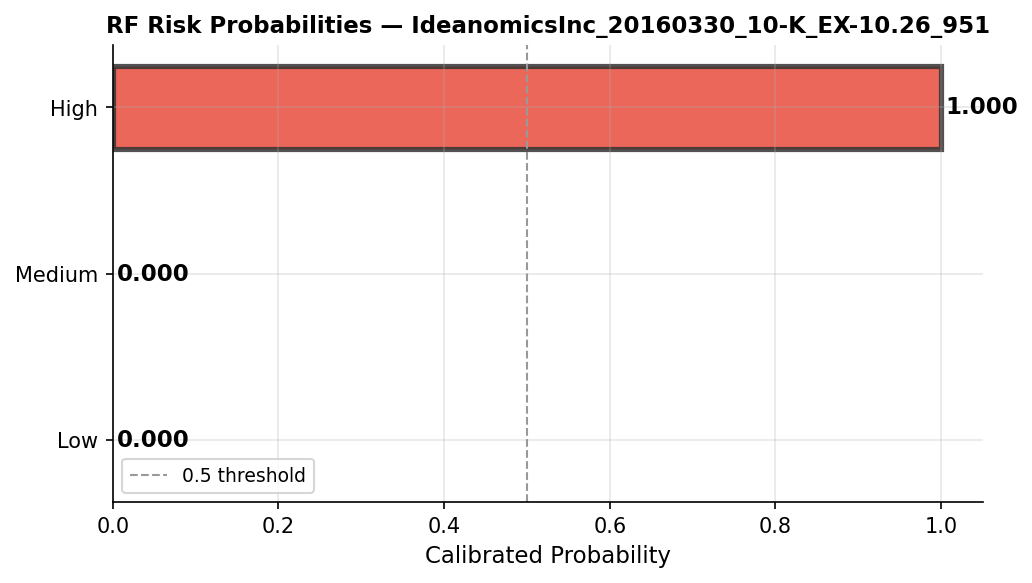
\includegraphics[width=\linewidth]{demo_probability_breakdown.png}
  \caption{Probability breakdown panel.}
\end{subfigure}
\caption{Explainability-oriented demonstration panels.}
\label{fig:demo}
\end{figure*}

\subsection{Bayesian network diagnostics (historical)}

\begin{figure*}[!t]
\centering
\begin{subfigure}[t]{0.48\textwidth}
  \centering
  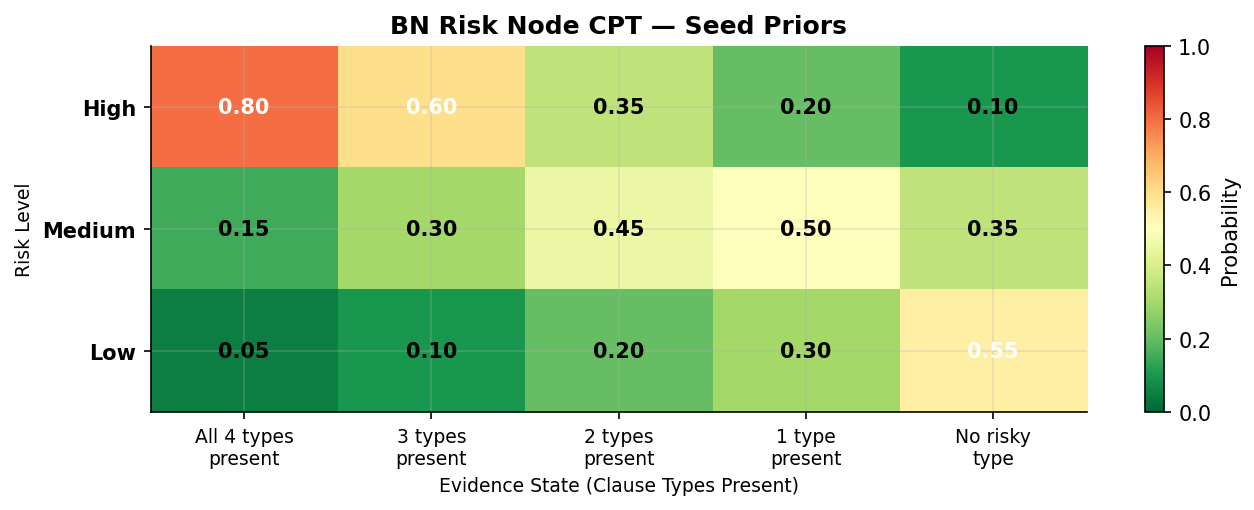
\includegraphics[width=\linewidth]{bn_cpt_heatmap.png}
  \caption{CPT heatmap.}
\end{subfigure}\hfill
\begin{subfigure}[t]{0.48\textwidth}
  \centering
  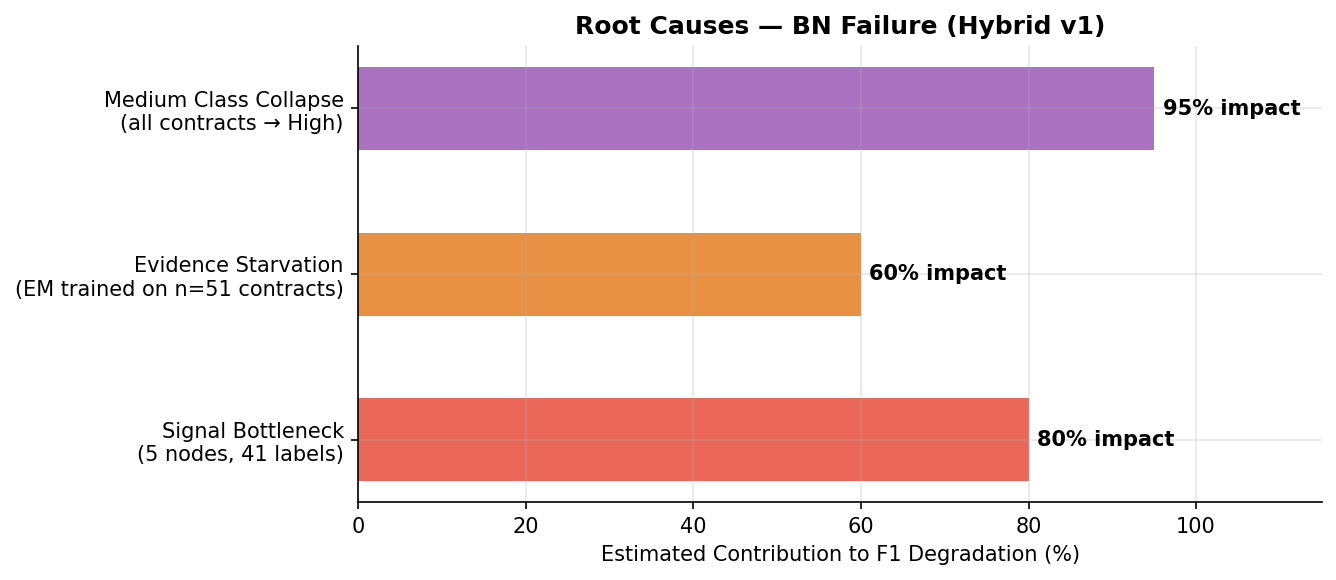
\includegraphics[width=\linewidth]{bn_failure_root_causes.png}
  \caption{Failure root-cause diagram.}
\end{subfigure}
\caption{BN-focused diagnostics supporting the starvation analysis in Section~\ref{sec:bn}.}
\label{fig:bndiags}
\end{figure*}

% =============================================================================
\section{Software Inventory and Entry Points}
\label{sec:scripts}
% =============================================================================

Table~\ref{tab:scripts} lists primary scripts referenced throughout experiments.

\begin{table}[!t]
\renewcommand{\arraystretch}{1.12}
\caption{Repository scripts and modules for training, evaluation, and analysis.}
\label{tab:scripts}
\centering
\footnotesize
\begin{tabularx}{\columnwidth}{@{}lX@{}}
\toprule
\textbf{Path} & \textbf{Purpose} \\
\midrule
\filepath{scripts/train_legal_bert_intensive.py} & Intensive Legal-BERT / LoRA training (Colab or local GPU). \\
\filepath{scripts/train_rf_reasoner.py} & Train and save \filepath{results/phase3/rf_reasoner.pkl}. \\
\filepath{scripts/threshold_sweep.py} & Coarse $\tau$ sweep with per-class F1 and average surviving labels. \\
\filepath{src/phase3/optimize_thresholds.py} & Dense $\tau$ sweep; recommends updated global floor. \\
\filepath{src/phase3/hybrid_eval_cli.py} & Contract-level hybrid evaluation CLI (\texttt{--rf-threshold}). \\
\filepath{src/phase3/hybrid_pipeline.py} & \texttt{AgastyaHybridPipeline} orchestration (RF primary when pickle present). \\
\filepath{src/phase3/hybrid_eval.py} & Dataset construction and metric wiring. \\
\filepath{src/phase3/failure_analysis.py} & Failure analysis utilities (uses $\tau=0.11$ in defaults). \\
\filepath{scripts/debug_legal_bert.py} & Qualitative Legal-BERT debugging. \\
\filepath{scripts/bert_clause_recall_diagnostics.py} & Clause recall diagnostics. \\
\filepath{scripts/package_colab_zip.sh} & Optional archive builder for Colab workflows. \\
\bottomrule
\end{tabularx}
\end{table}

% =============================================================================
\section{Reproducing the Headline Hybrid Metric}
\label{sec:repro}
% =============================================================================

From repository root with Phase~II encoder artifacts and \filepath{results/phase3/rf_reasoner.pkl} present:

\begin{lstlisting}
python -m src.phase3.hybrid_eval_cli --rf-threshold 0.11
\end{lstlisting}

Evaluation notebooks and CLI runs write fresh JSON to \filepath{reports/phase3/hybrid_eval.json} when configured to do so; always cite the JSON hash or timestamp used in the paper draft.

% =============================================================================
\section{Limitations and Reporting Caveats}
\label{sec:limits}
% =============================================================================

\begin{itemize}
  \item \textbf{Small contract sample:} $n=51$ contracts implies wide sampling uncertainty; Macro-F1 should be read as a \textbf{point estimate} on this slice, not a production SLA.
  \item \textbf{Derived risk labels:} Contract risk is deterministically mapped from Phase~II clause annotations; systematic errors in clause labels or mapping rules propagate verbatim.
  \item \textbf{BN code paths:} BN-related modules remain for research continuity but \textbf{do not} generate the primary metrics in Table~\ref{tab:hybrid}.
  \item \textbf{RoBERTa benchmark:} Documented failures reflect the specific fine-tuning and integration used; they should not be interpreted as universal impossibility results.
\end{itemize}

% =============================================================================
\section{Conclusion}
\label{sec:conc}
% =============================================================================

Agastya's documented path moves from lexical baselines through Legal-BERT with LoRA, attempts structured BN fusion, and ultimately standardizes on a calibrated random forest over the full clause label vector with an empirically tuned BERT confidence floor $\tau=0.11$. The BN stage provides interpretability insights but collapses quantitatively under CPT starvation; the RF stage recovers strong contract-level Macro-F1 ($0.866$ on the held-out contract construction) consistent with Tables~\ref{tab:hybrid}--\ref{tab:ablation}. Future work includes expanding contract coverage, richer uncertainty quantification, and optional reintroduction of structured models only when evidence pathways are statistically well supported.

\section*{Data and Code Availability}

All tables, scripts, and figure sources referenced here are located in the Agastya repository under \filepath{reports/phase3/}, \filepath{results/phase2/}, \filepath{results/phase3/}, \filepath{src/phase3/}, and \filepath{scripts/}.

\vspace{0.5em}
\noindent\textit{Revision note: regenerate numbers if \filepath{reports/phase3/hybrid_eval.json}, \filepath{results/phase2/results.json}, or \filepath{reports/phase3/phase_progression_summary.csv} change.}

% Optional: add IEEEtran bibliography when references.bib exists:
% \bibliographystyle{IEEEtran}
% \bibliography{IEEEabrv,references}

\end{document}
